\documentclass[1p]{elsarticle_modified}
%\bibliographystyle{elsarticle-num}

%\usepackage[colorlinks]{hyperref}
%\usepackage{abbrmath_seonhwa} %\Abb, \Ascr, \Acal ,\Abf, \Afrak
\usepackage{amsfonts}
\usepackage{amssymb}
\usepackage{amsmath}
\usepackage{amsthm}
\usepackage{scalefnt}
\usepackage{amsbsy}
\usepackage{kotex}
\usepackage{caption}
\usepackage{subfig}
\usepackage{color}
\usepackage{graphicx}
\usepackage{xcolor} %% white, black, red, green, blue, cyan, magenta, yellow
\usepackage{float}
\usepackage{setspace}
\usepackage{hyperref}

\usepackage{tikz}
\usetikzlibrary{arrows}

\usepackage{multirow}
\usepackage{array} % fixed length table
\usepackage{hhline}

%%%%%%%%%%%%%%%%%%%%%
\makeatletter
\renewcommand*\env@matrix[1][\arraystretch]{%
	\edef\arraystretch{#1}%
	\hskip -\arraycolsep
	\let\@ifnextchar\new@ifnextchar
	\array{*\c@MaxMatrixCols c}}
\makeatother %https://tex.stackexchange.com/questions/14071/how-can-i-increase-the-line-spacing-in-a-matrix
%%%%%%%%%%%%%%%

\usepackage[normalem]{ulem}

\newcommand{\msout}[1]{\ifmmode\text{\sout{\ensuremath{#1}}}\else\sout{#1}\fi}
%SOURCE: \msout is \stkout macro in https://tex.stackexchange.com/questions/20609/strikeout-in-math-mode

\newcommand{\cancel}[1]{
	\ifmmode
	{\color{red}\msout{#1}}
	\else
	{\color{red}\sout{#1}}
	\fi
}

\newcommand{\add}[1]{
	{\color{blue}\uwave{#1}}
}

\newcommand{\replace}[2]{
	\ifmmode
	{\color{red}\msout{#1}}{\color{blue}\uwave{#2}}
	\else
	{\color{red}\sout{#1}}{\color{blue}\uwave{#2}}
	\fi
}

\newcommand{\Sol}{\mathcal{S}} %segment
\newcommand{\D}{D} %diagram
\newcommand{\A}{\mathcal{A}} %arc


%%%%%%%%%%%%%%%%%%%%%%%%%%%%%5 test

\def\sl{\operatorname{\textup{SL}}(2,\Cbb)}
\def\psl{\operatorname{\textup{PSL}}(2,\Cbb)}
\def\quan{\mkern 1mu \triangleright \mkern 1mu}

\theoremstyle{definition}
\newtheorem{thm}{Theorem}[section]
\newtheorem{prop}[thm]{Proposition}
\newtheorem{lem}[thm]{Lemma}
\newtheorem{ques}[thm]{Question}
\newtheorem{cor}[thm]{Corollary}
\newtheorem{defn}[thm]{Definition}
\newtheorem{exam}[thm]{Example}
\newtheorem{rmk}[thm]{Remark}
\newtheorem{alg}[thm]{Algorithm}

\newcommand{\I}{\sqrt{-1}}
\begin{document}

%\begin{frontmatter}
%
%\title{Boundary parabolic representations of knots up to 8 crossings}
%
%%% Group authors per affiliation:
%\author{Yunhi Cho} 
%\address{Department of Mathematics, University of Seoul, Seoul, Korea}
%\ead{yhcho@uos.ac.kr}
%
%
%\author{Seonhwa Kim} %\fnref{s_kim}}
%\address{Center for Geometry and Physics, Institute for Basic Science, Pohang, 37673, Korea}
%\ead{ryeona17@ibs.re.kr}
%
%\author{Hyuk Kim}
%\address{Department of Mathematical Sciences, Seoul National University, Seoul 08826, Korea}
%\ead{hyukkim@snu.ac.kr}
%
%\author{Seokbeom Yoon}
%\address{Department of Mathematical Sciences, Seoul National University, Seoul, 08826,  Korea}
%\ead{sbyoon15@snu.ac.kr}
%
%\begin{abstract}
%We find all boundary parabolic representation of knots up to 8 crossings.
%
%\end{abstract}
%\begin{keyword}
%    \MSC[2010] 57M25 
%\end{keyword}
%
%\end{frontmatter}

%\linenumbers
%\tableofcontents
%
\newcommand\colored[1]{\textcolor{white}{\rule[-0.35ex]{0.8em}{1.4ex}}\kern-0.8em\color{red} #1}%
%\newcommand\colored[1]{\textcolor{white}{ #1}\kern-2.17ex	\textcolor{white}{ #1}\kern-1.81ex	\textcolor{white}{ #1}\kern-2.15ex\color{red}#1	}

{\Large $\underline{12a_{1080}~(K12a_{1080})}$}

\setlength{\tabcolsep}{10pt}
\renewcommand{\arraystretch}{1.6}
\vspace{1cm}\begin{tabular}{m{100pt}>{\centering\arraybackslash}m{274pt}}
\multirow{5}{120pt}{
	\centering
	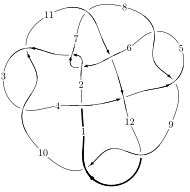
\includegraphics[width=112pt]{../../../GIT/diagram.site/Diagrams/png/1881_12a_1080.png}\\
\ \ \ A knot diagram\footnotemark}&
\allowdisplaybreaks
\textbf{Linearized knot diagam} \\
\cline{2-2}
 &
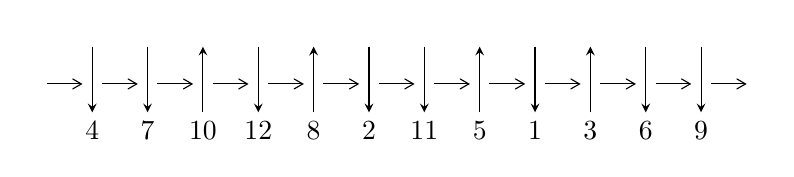
\begin{tikzpicture}[x=20pt, y=17pt]
	% nodes
	\node (C0) at (0, 0) {};
	\node (C1) at (1, 0) {};
	\node (C1U) at (1, +1) {};
	\node (C1D) at (1, -1) {4};

	\node (C2) at (2, 0) {};
	\node (C2U) at (2, +1) {};
	\node (C2D) at (2, -1) {7};

	\node (C3) at (3, 0) {};
	\node (C3U) at (3, +1) {};
	\node (C3D) at (3, -1) {10};

	\node (C4) at (4, 0) {};
	\node (C4U) at (4, +1) {};
	\node (C4D) at (4, -1) {12};

	\node (C5) at (5, 0) {};
	\node (C5U) at (5, +1) {};
	\node (C5D) at (5, -1) {8};

	\node (C6) at (6, 0) {};
	\node (C6U) at (6, +1) {};
	\node (C6D) at (6, -1) {2};

	\node (C7) at (7, 0) {};
	\node (C7U) at (7, +1) {};
	\node (C7D) at (7, -1) {11};

	\node (C8) at (8, 0) {};
	\node (C8U) at (8, +1) {};
	\node (C8D) at (8, -1) {5};

	\node (C9) at (9, 0) {};
	\node (C9U) at (9, +1) {};
	\node (C9D) at (9, -1) {1};

	\node (C10) at (10, 0) {};
	\node (C10U) at (10, +1) {};
	\node (C10D) at (10, -1) {3};

	\node (C11) at (11, 0) {};
	\node (C11U) at (11, +1) {};
	\node (C11D) at (11, -1) {6};

	\node (C12) at (12, 0) {};
	\node (C12U) at (12, +1) {};
	\node (C12D) at (12, -1) {9};
	\node (C13) at (13, 0) {};

	% arrows
	\draw[->,>={angle 60}]
	(C0) edge (C1) (C1) edge (C2) (C2) edge (C3) (C3) edge (C4) (C4) edge (C5) (C5) edge (C6) (C6) edge (C7) (C7) edge (C8) (C8) edge (C9) (C9) edge (C10) (C10) edge (C11) (C11) edge (C12) (C12) edge (C13) ;	\draw[->,>=stealth]
	(C1U) edge (C1D) (C2U) edge (C2D) (C3D) edge (C3U) (C4U) edge (C4D) (C5D) edge (C5U) (C6U) edge (C6D) (C7U) edge (C7D) (C8D) edge (C8U) (C9U) edge (C9D) (C10D) edge (C10U) (C11U) edge (C11D) (C12U) edge (C12D) ;
	\end{tikzpicture} \\
\hhline{~~} \\& 
\textbf{Solving Sequence} \\ \cline{2-2} 
 &
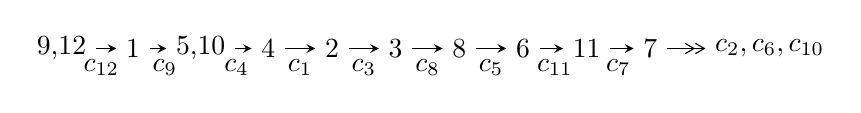
\begin{tikzpicture}[x=23pt, y=7pt]
	% node
	\node (A0) at (-1/8, 0) {9,12};
	\node (A1) at (1, 0) {1};
	\node (A2) at (33/16, 0) {5,10};
	\node (A3) at (25/8, 0) {4};
	\node (A4) at (33/8, 0) {2};
	\node (A5) at (41/8, 0) {3};
	\node (A6) at (49/8, 0) {8};
	\node (A7) at (57/8, 0) {6};
	\node (A8) at (65/8, 0) {11};
	\node (A9) at (73/8, 0) {7};
	\node (C1) at (1/2, -1) {$c_{12}$};
	\node (C2) at (3/2, -1) {$c_{9}$};
	\node (C3) at (21/8, -1) {$c_{4}$};
	\node (C4) at (29/8, -1) {$c_{1}$};
	\node (C5) at (37/8, -1) {$c_{3}$};
	\node (C6) at (45/8, -1) {$c_{8}$};
	\node (C7) at (53/8, -1) {$c_{5}$};
	\node (C8) at (61/8, -1) {$c_{11}$};
	\node (C9) at (69/8, -1) {$c_{7}$};
	\node (A10) at (11, 0) {$c_{2},c_{6},c_{10}$};

	% edge
	\draw[->,>=stealth]	
	(A0) edge (A1) (A1) edge (A2) (A2) edge (A3) (A3) edge (A4) (A4) edge (A5) (A5) edge (A6) (A6) edge (A7) (A7) edge (A8) (A8) edge (A9) ;
	\draw[->>,>={angle 60}]	
	(A9) edge (A10);
\end{tikzpicture} \\ 

\end{tabular} \\

\footnotetext{
The image of knot diagram is generated by the software ``\textbf{Draw programme}" developed by Andrew Bartholomew(\url{http://www.layer8.co.uk/maths/draw/index.htm\#Running-draw}), where we modified some parts for our purpose(\url{https://github.com/CATsTAILs/LinksPainter}).
}\phantom \\ \newline 
\centering \textbf{Ideals for irreducible components\footnotemark of $X_{\text{par}}$} 
 
\begin{align*}
I^u_{1}&=\langle 
5.71445\times10^{533} u^{129}-2.95703\times10^{534} u^{128}+\cdots+2.15300\times10^{534} b-3.92705\times10^{534},\\
\phantom{I^u_{1}}&\phantom{= \langle  }-7.74014\times10^{535} u^{129}+3.94800\times10^{536} u^{128}+\cdots+4.30600\times10^{534} a+6.77807\times10^{536},\\
\phantom{I^u_{1}}&\phantom{= \langle  }u^{130}-5 u^{129}+\cdots-6 u-1\rangle \\
I^u_{2}&=\langle 
5.03147\times10^{18} u^{28}-3.08387\times10^{19} u^{27}+\cdots+8.43939\times10^{18} b-1.04843\times10^{19},\\
\phantom{I^u_{2}}&\phantom{= \langle  }-1.85005\times10^{19} u^{28}+1.08812\times10^{20} u^{27}+\cdots+8.43939\times10^{18} a-3.82188\times10^{19},\;u^{29}-7 u^{28}+\cdots-5 u+1\rangle \\
I^u_{3}&=\langle 
b-1,\;a,\;u+1\rangle \\
\\
\end{align*}
\raggedright * 3 irreducible components of $\dim_{\mathbb{C}}=0$, with total 160 representations.\\
\footnotetext{All coefficients of polynomials are rational numbers. But the coefficients are sometimes approximated in decimal forms when there is not enough margin.}
\newpage
\renewcommand{\arraystretch}{1}
\centering \section*{I. $I^u_{1}= \langle 5.71\times10^{533} u^{129}-2.96\times10^{534} u^{128}+\cdots+2.15\times10^{534} b-3.93\times10^{534},\;-7.74\times10^{535} u^{129}+3.95\times10^{536} u^{128}+\cdots+4.31\times10^{534} a+6.78\times10^{536},\;u^{130}-5 u^{129}+\cdots-6 u-1 \rangle$}
\flushleft \textbf{(i) Arc colorings}\\
\begin{tabular}{m{7pt} m{180pt} m{7pt} m{180pt} }
\flushright $a_{9}=$&$\begin{pmatrix}0\\u\end{pmatrix}$ \\
\flushright $a_{12}=$&$\begin{pmatrix}1\\0\end{pmatrix}$ \\
\flushright $a_{1}=$&$\begin{pmatrix}1\\u^2\end{pmatrix}$ \\
\flushright $a_{5}=$&$\begin{pmatrix}17.9752 u^{129}-91.6859 u^{128}+\cdots+1038.28 u-157.410\\-0.265418 u^{129}+1.37345 u^{128}+\cdots+16.6270 u+1.82399\end{pmatrix}$ \\
\flushright $a_{10}=$&$\begin{pmatrix}- u\\- u^3+u\end{pmatrix}$ \\
\flushright $a_{4}=$&$\begin{pmatrix}17.7098 u^{129}-90.3124 u^{128}+\cdots+1054.91 u-155.586\\-0.265418 u^{129}+1.37345 u^{128}+\cdots+16.6270 u+1.82399\end{pmatrix}$ \\
\flushright $a_{2}=$&$\begin{pmatrix}-17.4445 u^{129}+88.8676 u^{128}+\cdots-86.8634 u+198.239\\0.479324 u^{129}-2.38693 u^{128}+\cdots+36.7566 u-3.63350\end{pmatrix}$ \\
\flushright $a_{3}=$&$\begin{pmatrix}17.6308 u^{129}-89.9462 u^{128}+\cdots+1047.76 u-153.876\\-0.0239336 u^{129}+0.128212 u^{128}+\cdots+23.5302 u+0.0849661\end{pmatrix}$ \\
\flushright $a_{8}=$&$\begin{pmatrix}9.43611 u^{129}-47.7722 u^{128}+\cdots+120.382 u-108.498\\-1.71518 u^{129}+8.55245 u^{128}+\cdots-88.2992 u+17.3088\end{pmatrix}$ \\
\flushright $a_{6}=$&$\begin{pmatrix}-10.5939 u^{129}+54.2944 u^{128}+\cdots-213.176 u+79.9416\\-0.898314 u^{129}+4.70501 u^{128}+\cdots-42.6358 u+8.95224\end{pmatrix}$ \\
\flushright $a_{11}=$&$\begin{pmatrix}-4.49629 u^{129}+22.7969 u^{128}+\cdots+151.904 u+56.6764\\1.62019 u^{129}-8.33401 u^{128}+\cdots+86.2625 u-16.5936\end{pmatrix}$ \\
\flushright $a_{7}=$&$\begin{pmatrix}-6.51812 u^{129}+33.3516 u^{128}+\cdots+552.533 u+85.7734\\0.0695352 u^{129}-0.309490 u^{128}+\cdots+29.3881 u+0.459493\end{pmatrix}$\\&\end{tabular}
\flushleft \textbf{(ii) Obstruction class $= -1$}\\~\\
\flushleft \textbf{(iii) Cusp Shapes $= -2.50096 u^{129}+12.6110 u^{128}+\cdots-163.450 u+16.2890$}\\~\\
\newpage\renewcommand{\arraystretch}{1}
\flushleft \textbf{(iv) u-Polynomials at the component}\newline \\
\begin{tabular}{m{50pt}|m{274pt}}
Crossings & \hspace{64pt}u-Polynomials at each crossing \\
\hline $$\begin{aligned}c_{1}\end{aligned}$$&$\begin{aligned}
&u^{130}-13 u^{129}+\cdots-179728050 u+10062098
\end{aligned}$\\
\hline $$\begin{aligned}c_{2},c_{6}\end{aligned}$$&$\begin{aligned}
&u^{130}-3 u^{129}+\cdots+8779 u-307
\end{aligned}$\\
\hline $$\begin{aligned}c_{3},c_{10}\end{aligned}$$&$\begin{aligned}
&u^{130}+6 u^{129}+\cdots+273801 u+6691
\end{aligned}$\\
\hline $$\begin{aligned}c_{4}\end{aligned}$$&$\begin{aligned}
&u^{130}+8 u^{129}+\cdots-32651759 u-16964329
\end{aligned}$\\
\hline $$\begin{aligned}c_{5},c_{8}\end{aligned}$$&$\begin{aligned}
&u^{130}+9 u^{129}+\cdots+6600 u+218
\end{aligned}$\\
\hline $$\begin{aligned}c_{7}\end{aligned}$$&$\begin{aligned}
&u^{130}+4 u^{129}+\cdots-3192063 u+4571051
\end{aligned}$\\
\hline $$\begin{aligned}c_{9},c_{12}\end{aligned}$$&$\begin{aligned}
&u^{130}-5 u^{129}+\cdots-6 u-1
\end{aligned}$\\
\hline $$\begin{aligned}c_{11}\end{aligned}$$&$\begin{aligned}
&u^{130}+12 u^{129}+\cdots+35960 u-90691
\end{aligned}$\\
\hline
\end{tabular}\\~\\
\newpage\renewcommand{\arraystretch}{1}
\flushleft \textbf{(v) Riley Polynomials at the component}\newline \\
\begin{tabular}{m{50pt}|m{274pt}}
Crossings & \hspace{64pt}Riley Polynomials at each crossing \\
\hline $$\begin{aligned}c_{1}\end{aligned}$$&$\begin{aligned}
&y^{130}-39 y^{129}+\cdots-12521051740895800 y+101245816161604
\end{aligned}$\\
\hline $$\begin{aligned}c_{2},c_{6}\end{aligned}$$&$\begin{aligned}
&y^{130}-87 y^{129}+\cdots-162306321 y+94249
\end{aligned}$\\
\hline $$\begin{aligned}c_{3},c_{10}\end{aligned}$$&$\begin{aligned}
&y^{130}+34 y^{129}+\cdots-59906322757 y+44769481
\end{aligned}$\\
\hline $$\begin{aligned}c_{4}\end{aligned}$$&$\begin{aligned}
&y^{130}-128 y^{129}+\cdots-5434457919023257 y+287788458420241
\end{aligned}$\\
\hline $$\begin{aligned}c_{5},c_{8}\end{aligned}$$&$\begin{aligned}
&y^{130}+111 y^{129}+\cdots-8958604 y+47524
\end{aligned}$\\
\hline $$\begin{aligned}c_{7}\end{aligned}$$&$\begin{aligned}
&y^{130}-70 y^{129}+\cdots-3447337940891247 y+20894507244601
\end{aligned}$\\
\hline $$\begin{aligned}c_{9},c_{12}\end{aligned}$$&$\begin{aligned}
&y^{130}-115 y^{129}+\cdots-68 y+1
\end{aligned}$\\
\hline $$\begin{aligned}c_{11}\end{aligned}$$&$\begin{aligned}
&y^{130}-96 y^{129}+\cdots+30998315860 y+8224857481
\end{aligned}$\\
\hline
\end{tabular}\\~\\
\newpage\flushleft \textbf{(vi) Complex Volumes and Cusp Shapes}
$$\begin{array}{c|c|c}  
\text{Solutions to }I^u_{1}& \I (\text{vol} + \sqrt{-1}CS) & \text{Cusp shape}\\
 \hline 
\begin{aligned}
u &= -1.00202\phantom{ +0.000000I} \\
a &= -0.0616349\phantom{ +0.000000I} \\
b &= -8.97342\phantom{ +0.000000I}\end{aligned}
 & -3.29193\phantom{ +0.000000I} & \phantom{-0.000000 } 0 \\ \hline\begin{aligned}
u &= -0.073491 + 0.987925 I \\
a &= \phantom{-}1.315450 - 0.395938 I \\
b &= -0.889853 + 0.641878 I\end{aligned}
 & -3.61027 + 7.42880 I & \phantom{-0.000000 } 0 \\ \hline\begin{aligned}
u &= -0.073491 - 0.987925 I \\
a &= \phantom{-}1.315450 + 0.395938 I \\
b &= -0.889853 - 0.641878 I\end{aligned}
 & -3.61027 - 7.42880 I & \phantom{-0.000000 } 0 \\ \hline\begin{aligned}
u &= -0.409840 + 0.896900 I \\
a &= \phantom{-}0.883868 - 0.533532 I \\
b &= -0.763894 + 0.603595 I\end{aligned}
 & -1.69773 + 2.65884 I & \phantom{-0.000000 } 0 \\ \hline\begin{aligned}
u &= -0.409840 - 0.896900 I \\
a &= \phantom{-}0.883868 + 0.533532 I \\
b &= -0.763894 - 0.603595 I\end{aligned}
 & -1.69773 - 2.65884 I & \phantom{-0.000000 } 0 \\ \hline\begin{aligned}
u &= -0.020637 + 0.967032 I \\
a &= -0.084685 + 0.964659 I \\
b &= -0.375576 - 0.657852 I\end{aligned}
 & -0.50407 - 1.50340 I & \phantom{-0.000000 } 0 \\ \hline\begin{aligned}
u &= -0.020637 - 0.967032 I \\
a &= -0.084685 - 0.964659 I \\
b &= -0.375576 + 0.657852 I\end{aligned}
 & -0.50407 + 1.50340 I & \phantom{-0.000000 } 0 \\ \hline\begin{aligned}
u &= -0.129553 + 0.930254 I \\
a &= -1.217950 + 0.545282 I \\
b &= \phantom{-}0.727114 - 0.502909 I\end{aligned}
 & -0.51607 + 3.67076 I & \phantom{-0.000000 } 0 \\ \hline\begin{aligned}
u &= -0.129553 - 0.930254 I \\
a &= -1.217950 - 0.545282 I \\
b &= \phantom{-}0.727114 + 0.502909 I\end{aligned}
 & -0.51607 - 3.67076 I & \phantom{-0.000000 } 0 \\ \hline\begin{aligned}
u &= \phantom{-}0.090422 + 0.924094 I \\
a &= \phantom{-}0.069738 - 1.052160 I \\
b &= \phantom{-}0.488227 + 0.892671 I\end{aligned}
 & -4.45289 - 8.08828 I & \phantom{-0.000000 } 0\\
 \hline 
 \end{array}$$\newpage$$\begin{array}{c|c|c}  
\text{Solutions to }I^u_{1}& \I (\text{vol} + \sqrt{-1}CS) & \text{Cusp shape}\\
 \hline 
\begin{aligned}
u &= \phantom{-}0.090422 - 0.924094 I \\
a &= \phantom{-}0.069738 + 1.052160 I \\
b &= \phantom{-}0.488227 - 0.892671 I\end{aligned}
 & -4.45289 + 8.08828 I & \phantom{-0.000000 } 0 \\ \hline\begin{aligned}
u &= -1.07910\phantom{ +0.000000I} \\
a &= -0.316887\phantom{ +0.000000I} \\
b &= -0.845615\phantom{ +0.000000I}\end{aligned}
 & -1.80194\phantom{ +0.000000I} & \phantom{-0.000000 } 0 \\ \hline\begin{aligned}
u &= -1.083850 + 0.160880 I \\
a &= \phantom{-}0.597938 - 0.242020 I \\
b &= \phantom{-}0.636688 + 0.640814 I\end{aligned}
 & -2.11300 + 0.79916 I & \phantom{-0.000000 } 0 \\ \hline\begin{aligned}
u &= -1.083850 - 0.160880 I \\
a &= \phantom{-}0.597938 + 0.242020 I \\
b &= \phantom{-}0.636688 - 0.640814 I\end{aligned}
 & -2.11300 - 0.79916 I & \phantom{-0.000000 } 0 \\ \hline\begin{aligned}
u &= -0.242844 + 0.845324 I \\
a &= -0.995175 + 0.758224 I \\
b &= \phantom{-}1.088130 - 0.680843 I\end{aligned}
 & -3.62197 + 5.01079 I & \phantom{-0.000000 } 0 \\ \hline\begin{aligned}
u &= -0.242844 - 0.845324 I \\
a &= -0.995175 - 0.758224 I \\
b &= \phantom{-}1.088130 + 0.680843 I\end{aligned}
 & -3.62197 - 5.01079 I & \phantom{-0.000000 } 0 \\ \hline\begin{aligned}
u &= \phantom{-}1.095850 + 0.271330 I \\
a &= -0.789504 + 0.483119 I \\
b &= -0.658536 - 0.592176 I\end{aligned}
 & \phantom{-}0.31867 - 3.20607 I & \phantom{-0.000000 } 0 \\ \hline\begin{aligned}
u &= \phantom{-}1.095850 - 0.271330 I \\
a &= -0.789504 - 0.483119 I \\
b &= -0.658536 + 0.592176 I\end{aligned}
 & \phantom{-}0.31867 + 3.20607 I & \phantom{-0.000000 } 0 \\ \hline\begin{aligned}
u &= \phantom{-}1.097640 + 0.274588 I \\
a &= -0.12884 + 1.41473 I \\
b &= -0.658414 - 0.715748 I\end{aligned}
 & -2.84987 - 4.21682 I & \phantom{-0.000000 } 0 \\ \hline\begin{aligned}
u &= \phantom{-}1.097640 - 0.274588 I \\
a &= -0.12884 - 1.41473 I \\
b &= -0.658414 + 0.715748 I\end{aligned}
 & -2.84987 + 4.21682 I & \phantom{-0.000000 } 0\\
 \hline 
 \end{array}$$\newpage$$\begin{array}{c|c|c}  
\text{Solutions to }I^u_{1}& \I (\text{vol} + \sqrt{-1}CS) & \text{Cusp shape}\\
 \hline 
\begin{aligned}
u &= -1.119590 + 0.200790 I \\
a &= -0.155962 + 1.179580 I \\
b &= \phantom{-}2.88822 - 0.94863 I\end{aligned}
 & -8.11010 + 0.62872 I & \phantom{-0.000000 } 0 \\ \hline\begin{aligned}
u &= -1.119590 - 0.200790 I \\
a &= -0.155962 - 1.179580 I \\
b &= \phantom{-}2.88822 + 0.94863 I\end{aligned}
 & -8.11010 - 0.62872 I & \phantom{-0.000000 } 0 \\ \hline\begin{aligned}
u &= \phantom{-}1.150330 + 0.007367 I \\
a &= \phantom{-}0.572667 - 1.059770 I \\
b &= \phantom{-}0.689821 + 0.179403 I\end{aligned}
 & -4.77689 + 2.09602 I & \phantom{-0.000000 } 0 \\ \hline\begin{aligned}
u &= \phantom{-}1.150330 - 0.007367 I \\
a &= \phantom{-}0.572667 + 1.059770 I \\
b &= \phantom{-}0.689821 - 0.179403 I\end{aligned}
 & -4.77689 - 2.09602 I & \phantom{-0.000000 } 0 \\ \hline\begin{aligned}
u &= -1.136690 + 0.223145 I \\
a &= -0.404583 + 0.204210 I \\
b &= -0.237139 + 0.768520 I\end{aligned}
 & -2.74861 - 0.75488 I & \phantom{-0.000000 } 0 \\ \hline\begin{aligned}
u &= -1.136690 - 0.223145 I \\
a &= -0.404583 - 0.204210 I \\
b &= -0.237139 - 0.768520 I\end{aligned}
 & -2.74861 + 0.75488 I & \phantom{-0.000000 } 0 \\ \hline\begin{aligned}
u &= \phantom{-}1.18620\phantom{ +0.000000I} \\
a &= \phantom{-}1.12730\phantom{ +0.000000I} \\
b &= \phantom{-}0.812482\phantom{ +0.000000I}\end{aligned}
 & -5.51674\phantom{ +0.000000I} & \phantom{-0.000000 } 0 \\ \hline\begin{aligned}
u &= -1.224080 + 0.092709 I \\
a &= -1.06586 + 1.58713 I \\
b &= -0.440715 - 0.317754 I\end{aligned}
 & -11.92840 + 3.71446 I & \phantom{-0.000000 } 0 \\ \hline\begin{aligned}
u &= -1.224080 - 0.092709 I \\
a &= -1.06586 - 1.58713 I \\
b &= -0.440715 + 0.317754 I\end{aligned}
 & -11.92840 - 3.71446 I & \phantom{-0.000000 } 0 \\ \hline\begin{aligned}
u &= \phantom{-}1.194690 + 0.331291 I \\
a &= \phantom{-}0.648812 - 0.429668 I \\
b &= \phantom{-}0.921396 + 0.752959 I\end{aligned}
 & -2.49703 - 7.75580 I & \phantom{-0.000000 } 0\\
 \hline 
 \end{array}$$\newpage$$\begin{array}{c|c|c}  
\text{Solutions to }I^u_{1}& \I (\text{vol} + \sqrt{-1}CS) & \text{Cusp shape}\\
 \hline 
\begin{aligned}
u &= \phantom{-}1.194690 - 0.331291 I \\
a &= \phantom{-}0.648812 + 0.429668 I \\
b &= \phantom{-}0.921396 - 0.752959 I\end{aligned}
 & -2.49703 + 7.75580 I & \phantom{-0.000000 } 0 \\ \hline\begin{aligned}
u &= -0.030993 + 0.755408 I \\
a &= -0.144627 - 0.837090 I \\
b &= \phantom{-}0.752383 + 0.319406 I\end{aligned}
 & -6.21610 + 3.71666 I & \phantom{-0.000000 } 0 \\ \hline\begin{aligned}
u &= -0.030993 - 0.755408 I \\
a &= -0.144627 + 0.837090 I \\
b &= \phantom{-}0.752383 - 0.319406 I\end{aligned}
 & -6.21610 - 3.71666 I & \phantom{-0.000000 } 0 \\ \hline\begin{aligned}
u &= -1.253630 + 0.015548 I \\
a &= \phantom{-}0.384371 - 0.207385 I \\
b &= \phantom{-}0.836924 - 0.860718 I\end{aligned}
 & -2.67890 + 1.86876 I & \phantom{-0.000000 } 0 \\ \hline\begin{aligned}
u &= -1.253630 - 0.015548 I \\
a &= \phantom{-}0.384371 + 0.207385 I \\
b &= \phantom{-}0.836924 + 0.860718 I\end{aligned}
 & -2.67890 - 1.86876 I & \phantom{-0.000000 } 0 \\ \hline\begin{aligned}
u &= -1.118880 + 0.570219 I \\
a &= \phantom{-}0.390866 - 0.720429 I \\
b &= -0.934232 - 0.180625 I\end{aligned}
 & -6.03411 + 0.01480 I & \phantom{-0.000000 } 0 \\ \hline\begin{aligned}
u &= -1.118880 - 0.570219 I \\
a &= \phantom{-}0.390866 + 0.720429 I \\
b &= -0.934232 + 0.180625 I\end{aligned}
 & -6.03411 - 0.01480 I & \phantom{-0.000000 } 0 \\ \hline\begin{aligned}
u &= -0.194122 + 0.709389 I \\
a &= \phantom{-}1.51868 - 0.76656 I \\
b &= -1.156460 - 0.029029 I\end{aligned}
 & -5.55815 + 2.85770 I & \phantom{-0.000000 } 0 \\ \hline\begin{aligned}
u &= -0.194122 - 0.709389 I \\
a &= \phantom{-}1.51868 + 0.76656 I \\
b &= -1.156460 + 0.029029 I\end{aligned}
 & -5.55815 - 2.85770 I & \phantom{-0.000000 } 0 \\ \hline\begin{aligned}
u &= -1.271440 + 0.012123 I \\
a &= \phantom{-}0.335518 + 1.315410 I \\
b &= \phantom{-}0.985026 - 0.992068 I\end{aligned}
 & -9.42887 + 2.93806 I & \phantom{-0.000000 } 0\\
 \hline 
 \end{array}$$\newpage$$\begin{array}{c|c|c}  
\text{Solutions to }I^u_{1}& \I (\text{vol} + \sqrt{-1}CS) & \text{Cusp shape}\\
 \hline 
\begin{aligned}
u &= -1.271440 - 0.012123 I \\
a &= \phantom{-}0.335518 - 1.315410 I \\
b &= \phantom{-}0.985026 + 0.992068 I\end{aligned}
 & -9.42887 - 2.93806 I & \phantom{-0.000000 } 0 \\ \hline\begin{aligned}
u &= \phantom{-}0.440963 + 1.195240 I \\
a &= -0.855898 - 0.678673 I \\
b &= \phantom{-}0.871594 + 0.698929 I\end{aligned}
 & -8.7020 - 13.0723 I & \phantom{-0.000000 } 0 \\ \hline\begin{aligned}
u &= \phantom{-}0.440963 - 1.195240 I \\
a &= -0.855898 + 0.678673 I \\
b &= \phantom{-}0.871594 - 0.698929 I\end{aligned}
 & -8.7020 + 13.0723 I & \phantom{-0.000000 } 0 \\ \hline\begin{aligned}
u &= -1.249240 + 0.285238 I \\
a &= -1.024480 - 0.471633 I \\
b &= -0.859403 + 0.184929 I\end{aligned}
 & -9.97413 - 0.00960 I & \phantom{-0.000000 } 0 \\ \hline\begin{aligned}
u &= -1.249240 - 0.285238 I \\
a &= -1.024480 + 0.471633 I \\
b &= -0.859403 - 0.184929 I\end{aligned}
 & -9.97413 + 0.00960 I & \phantom{-0.000000 } 0 \\ \hline\begin{aligned}
u &= \phantom{-}0.060570 + 0.706728 I \\
a &= \phantom{-}0.269155 - 0.894738 I \\
b &= -0.356989 + 0.978877 I\end{aligned}
 & \phantom{-}0.95733 + 3.92673 I & \phantom{-0.000000 } 0 \\ \hline\begin{aligned}
u &= \phantom{-}0.060570 - 0.706728 I \\
a &= \phantom{-}0.269155 + 0.894738 I \\
b &= -0.356989 - 0.978877 I\end{aligned}
 & \phantom{-}0.95733 - 3.92673 I & \phantom{-0.000000 } 0 \\ \hline\begin{aligned}
u &= \phantom{-}0.254318 + 0.660041 I \\
a &= -0.224910 + 1.035090 I \\
b &= \phantom{-}0.121313 - 0.854569 I\end{aligned}
 & \phantom{-}2.84269 - 0.32651 I & \phantom{-0.000000 } 0 \\ \hline\begin{aligned}
u &= \phantom{-}0.254318 - 0.660041 I \\
a &= -0.224910 - 1.035090 I \\
b &= \phantom{-}0.121313 + 0.854569 I\end{aligned}
 & \phantom{-}2.84269 + 0.32651 I & \phantom{-0.000000 } 0 \\ \hline\begin{aligned}
u &= \phantom{-}1.311880 + 0.020045 I \\
a &= \phantom{-}0.012950 - 0.962013 I \\
b &= -1.77191 + 1.66222 I\end{aligned}
 & -13.9433 - 7.8812 I & \phantom{-0.000000 } 0\\
 \hline 
 \end{array}$$\newpage$$\begin{array}{c|c|c}  
\text{Solutions to }I^u_{1}& \I (\text{vol} + \sqrt{-1}CS) & \text{Cusp shape}\\
 \hline 
\begin{aligned}
u &= \phantom{-}1.311880 - 0.020045 I \\
a &= \phantom{-}0.012950 + 0.962013 I \\
b &= -1.77191 - 1.66222 I\end{aligned}
 & -13.9433 + 7.8812 I & \phantom{-0.000000 } 0 \\ \hline\begin{aligned}
u &= -1.328540 + 0.000938 I \\
a &= -0.503466 - 1.139700 I \\
b &= -1.279620 + 0.498610 I\end{aligned}
 & -14.1933 + 7.5974 I & \phantom{-0.000000 } 0 \\ \hline\begin{aligned}
u &= -1.328540 - 0.000938 I \\
a &= -0.503466 + 1.139700 I \\
b &= -1.279620 - 0.498610 I\end{aligned}
 & -14.1933 - 7.5974 I & \phantom{-0.000000 } 0 \\ \hline\begin{aligned}
u &= \phantom{-}1.334430 + 0.011122 I \\
a &= \phantom{-}0.033605 + 0.980534 I \\
b &= \phantom{-}1.42537 - 1.26333 I\end{aligned}
 & -10.35500 - 2.89604 I & \phantom{-0.000000 } 0 \\ \hline\begin{aligned}
u &= \phantom{-}1.334430 - 0.011122 I \\
a &= \phantom{-}0.033605 - 0.980534 I \\
b &= \phantom{-}1.42537 + 1.26333 I\end{aligned}
 & -10.35500 + 2.89604 I & \phantom{-0.000000 } 0 \\ \hline\begin{aligned}
u &= -1.330320 + 0.170812 I \\
a &= \phantom{-}0.079576 + 0.950102 I \\
b &= \phantom{-}1.82229 - 1.55223 I\end{aligned}
 & -5.94349 + 4.90505 I & \phantom{-0.000000 } 0 \\ \hline\begin{aligned}
u &= -1.330320 - 0.170812 I \\
a &= \phantom{-}0.079576 - 0.950102 I \\
b &= \phantom{-}1.82229 + 1.55223 I\end{aligned}
 & -5.94349 - 4.90505 I & \phantom{-0.000000 } 0 \\ \hline\begin{aligned}
u &= \phantom{-}1.328030 + 0.197054 I \\
a &= \phantom{-}0.576524 + 0.293758 I \\
b &= \phantom{-}0.864753 + 0.387823 I\end{aligned}
 & -5.00318 - 3.21559 I & \phantom{-0.000000 } 0 \\ \hline\begin{aligned}
u &= \phantom{-}1.328030 - 0.197054 I \\
a &= \phantom{-}0.576524 - 0.293758 I \\
b &= \phantom{-}0.864753 - 0.387823 I\end{aligned}
 & -5.00318 + 3.21559 I & \phantom{-0.000000 } 0 \\ \hline\begin{aligned}
u &= -1.281040 + 0.418549 I \\
a &= \phantom{-}0.809033 + 0.672759 I \\
b &= \phantom{-}0.690595 - 0.535196 I\end{aligned}
 & -4.44925 + 6.36446 I & \phantom{-0.000000 } 0\\
 \hline 
 \end{array}$$\newpage$$\begin{array}{c|c|c}  
\text{Solutions to }I^u_{1}& \I (\text{vol} + \sqrt{-1}CS) & \text{Cusp shape}\\
 \hline 
\begin{aligned}
u &= -1.281040 - 0.418549 I \\
a &= \phantom{-}0.809033 - 0.672759 I \\
b &= \phantom{-}0.690595 + 0.535196 I\end{aligned}
 & -4.44925 - 6.36446 I & \phantom{-0.000000 } 0 \\ \hline\begin{aligned}
u &= \phantom{-}1.341430 + 0.190127 I \\
a &= -0.827371 - 0.207179 I \\
b &= -1.002280 - 0.480499 I\end{aligned}
 & -6.40527 - 3.33195 I & \phantom{-0.000000 } 0 \\ \hline\begin{aligned}
u &= \phantom{-}1.341430 - 0.190127 I \\
a &= -0.827371 + 0.207179 I \\
b &= -1.002280 + 0.480499 I\end{aligned}
 & -6.40527 + 3.33195 I & \phantom{-0.000000 } 0 \\ \hline\begin{aligned}
u &= \phantom{-}1.320880 + 0.332965 I \\
a &= \phantom{-}0.0018459 + 0.1399580 I \\
b &= -1.341270 + 0.332724 I\end{aligned}
 & -10.47680 - 7.70288 I & \phantom{-0.000000 } 0 \\ \hline\begin{aligned}
u &= \phantom{-}1.320880 - 0.332965 I \\
a &= \phantom{-}0.0018459 - 0.1399580 I \\
b &= -1.341270 - 0.332724 I\end{aligned}
 & -10.47680 + 7.70288 I & \phantom{-0.000000 } 0 \\ \hline\begin{aligned}
u &= -1.352890 + 0.221980 I \\
a &= \phantom{-}0.015406 - 0.853772 I \\
b &= -1.26724 + 1.43738 I\end{aligned}
 & -5.20381 + 1.63050 I & \phantom{-0.000000 } 0 \\ \hline\begin{aligned}
u &= -1.352890 - 0.221980 I \\
a &= \phantom{-}0.015406 + 0.853772 I \\
b &= -1.26724 - 1.43738 I\end{aligned}
 & -5.20381 - 1.63050 I & \phantom{-0.000000 } 0 \\ \hline\begin{aligned}
u &= -1.354340 + 0.278982 I \\
a &= \phantom{-}0.083985 - 0.858763 I \\
b &= -1.23852 + 1.09364 I\end{aligned}
 & -5.20629 + 1.68465 I & \phantom{-0.000000 } 0 \\ \hline\begin{aligned}
u &= -1.354340 - 0.278982 I \\
a &= \phantom{-}0.083985 + 0.858763 I \\
b &= -1.23852 - 1.09364 I\end{aligned}
 & -5.20629 - 1.68465 I & \phantom{-0.000000 } 0 \\ \hline\begin{aligned}
u &= \phantom{-}1.355230 + 0.288926 I \\
a &= \phantom{-}0.158142 - 1.109720 I \\
b &= \phantom{-}1.26542 + 0.68333 I\end{aligned}
 & -10.43720 - 6.44469 I & \phantom{-0.000000 } 0\\
 \hline 
 \end{array}$$\newpage$$\begin{array}{c|c|c}  
\text{Solutions to }I^u_{1}& \I (\text{vol} + \sqrt{-1}CS) & \text{Cusp shape}\\
 \hline 
\begin{aligned}
u &= \phantom{-}1.355230 - 0.288926 I \\
a &= \phantom{-}0.158142 + 1.109720 I \\
b &= \phantom{-}1.26542 - 0.68333 I\end{aligned}
 & -10.43720 + 6.44469 I & \phantom{-0.000000 } 0 \\ \hline\begin{aligned}
u &= \phantom{-}1.387820 + 0.051455 I \\
a &= -0.007288 - 1.052230 I \\
b &= -0.58780 + 1.54672 I\end{aligned}
 & -14.1274 + 1.4151 I & \phantom{-0.000000 } 0 \\ \hline\begin{aligned}
u &= \phantom{-}1.387820 - 0.051455 I \\
a &= -0.007288 + 1.052230 I \\
b &= -0.58780 - 1.54672 I\end{aligned}
 & -14.1274 - 1.4151 I & \phantom{-0.000000 } 0 \\ \hline\begin{aligned}
u &= -1.336980 + 0.388354 I \\
a &= -0.802035 - 0.511974 I \\
b &= -0.835602 + 0.664222 I\end{aligned}
 & -8.9382 + 12.7310 I & \phantom{-0.000000 } 0 \\ \hline\begin{aligned}
u &= -1.336980 - 0.388354 I \\
a &= -0.802035 + 0.511974 I \\
b &= -0.835602 - 0.664222 I\end{aligned}
 & -8.9382 - 12.7310 I & \phantom{-0.000000 } 0 \\ \hline\begin{aligned}
u &= -0.575430 + 0.191897 I \\
a &= -0.75266 + 2.21488 I \\
b &= \phantom{-}0.95730 + 1.45363 I\end{aligned}
 & -7.66415 + 0.37111 I & \phantom{-0.000000 } 0 \\ \hline\begin{aligned}
u &= -0.575430 - 0.191897 I \\
a &= -0.75266 - 2.21488 I \\
b &= \phantom{-}0.95730 - 1.45363 I\end{aligned}
 & -7.66415 - 0.37111 I & \phantom{-0.000000 } 0 \\ \hline\begin{aligned}
u &= \phantom{-}1.342190 + 0.378213 I \\
a &= -0.013183 + 1.071910 I \\
b &= -1.41597 - 1.12995 I\end{aligned}
 & -5.11178 - 8.25838 I & \phantom{-0.000000 } 0 \\ \hline\begin{aligned}
u &= \phantom{-}1.342190 - 0.378213 I \\
a &= -0.013183 - 1.071910 I \\
b &= -1.41597 + 1.12995 I\end{aligned}
 & -5.11178 + 8.25838 I & \phantom{-0.000000 } 0 \\ \hline\begin{aligned}
u &= \phantom{-}1.338300 + 0.420027 I \\
a &= -0.056252 - 1.064140 I \\
b &= \phantom{-}1.65777 + 1.17573 I\end{aligned}
 & -8.0509 - 12.3800 I & \phantom{-0.000000 } 0\\
 \hline 
 \end{array}$$\newpage$$\begin{array}{c|c|c}  
\text{Solutions to }I^u_{1}& \I (\text{vol} + \sqrt{-1}CS) & \text{Cusp shape}\\
 \hline 
\begin{aligned}
u &= \phantom{-}1.338300 - 0.420027 I \\
a &= -0.056252 + 1.064140 I \\
b &= \phantom{-}1.65777 - 1.17573 I\end{aligned}
 & -8.0509 + 12.3800 I & \phantom{-0.000000 } 0 \\ \hline\begin{aligned}
u &= \phantom{-}1.41920 + 0.02261 I \\
a &= -0.053861 + 1.115730 I \\
b &= -0.455069 - 0.662436 I\end{aligned}
 & -13.99120 - 0.99445 I & \phantom{-0.000000 } 0 \\ \hline\begin{aligned}
u &= \phantom{-}1.41920 - 0.02261 I \\
a &= -0.053861 - 1.115730 I \\
b &= -0.455069 + 0.662436 I\end{aligned}
 & -13.99120 + 0.99445 I & \phantom{-0.000000 } 0 \\ \hline\begin{aligned}
u &= \phantom{-}1.41300 + 0.29459 I \\
a &= \phantom{-}0.130921 + 0.119386 I \\
b &= \phantom{-}0.810368 - 0.056158 I\end{aligned}
 & -5.67729 - 3.56833 I & \phantom{-0.000000 } 0 \\ \hline\begin{aligned}
u &= \phantom{-}1.41300 - 0.29459 I \\
a &= \phantom{-}0.130921 - 0.119386 I \\
b &= \phantom{-}0.810368 + 0.056158 I\end{aligned}
 & -5.67729 + 3.56833 I & \phantom{-0.000000 } 0 \\ \hline\begin{aligned}
u &= \phantom{-}1.40445 + 0.33837 I \\
a &= -0.195996 + 0.878968 I \\
b &= -1.68456 - 0.82654 I\end{aligned}
 & -8.84937 - 9.24827 I & \phantom{-0.000000 } 0 \\ \hline\begin{aligned}
u &= \phantom{-}1.40445 - 0.33837 I \\
a &= -0.195996 - 0.878968 I \\
b &= -1.68456 + 0.82654 I\end{aligned}
 & -8.84937 + 9.24827 I & \phantom{-0.000000 } 0 \\ \hline\begin{aligned}
u &= \phantom{-}0.157642 + 0.516695 I \\
a &= -1.74025 - 0.24932 I \\
b &= \phantom{-}0.511814 + 0.349407 I\end{aligned}
 & -0.530702 + 1.255080 I & -4.00000 - 3.64281 I \\ \hline\begin{aligned}
u &= \phantom{-}0.157642 - 0.516695 I \\
a &= -1.74025 + 0.24932 I \\
b &= \phantom{-}0.511814 - 0.349407 I\end{aligned}
 & -0.530702 - 1.255080 I & -4.00000 + 3.64281 I \\ \hline\begin{aligned}
u &= \phantom{-}0.62953 + 1.33910 I \\
a &= \phantom{-}0.632615 + 0.613599 I \\
b &= -0.668136 - 0.589000 I\end{aligned}
 & -4.04361 - 6.29930 I & \phantom{-0.000000 } 0\\
 \hline 
 \end{array}$$\newpage$$\begin{array}{c|c|c}  
\text{Solutions to }I^u_{1}& \I (\text{vol} + \sqrt{-1}CS) & \text{Cusp shape}\\
 \hline 
\begin{aligned}
u &= \phantom{-}0.62953 - 1.33910 I \\
a &= \phantom{-}0.632615 - 0.613599 I \\
b &= -0.668136 + 0.589000 I\end{aligned}
 & -4.04361 + 6.29930 I & \phantom{-0.000000 } 0 \\ \hline\begin{aligned}
u &= \phantom{-}1.44298 + 0.34787 I \\
a &= \phantom{-}0.027603 - 0.837185 I \\
b &= \phantom{-}1.63762 + 1.01601 I\end{aligned}
 & -7.47543 - 7.09269 I & \phantom{-0.000000 } 0 \\ \hline\begin{aligned}
u &= \phantom{-}1.44298 - 0.34787 I \\
a &= \phantom{-}0.027603 + 0.837185 I \\
b &= \phantom{-}1.63762 - 1.01601 I\end{aligned}
 & -7.47543 + 7.09269 I & \phantom{-0.000000 } 0 \\ \hline\begin{aligned}
u &= -0.020568 + 0.493316 I \\
a &= -1.36949 - 0.75216 I \\
b &= \phantom{-}0.055730 + 0.980040 I\end{aligned}
 & -0.690944 + 0.710546 I & -5.10637 + 0. I\phantom{ +0.000000I} \\ \hline\begin{aligned}
u &= -0.020568 - 0.493316 I \\
a &= -1.36949 + 0.75216 I \\
b &= \phantom{-}0.055730 - 0.980040 I\end{aligned}
 & -0.690944 - 0.710546 I & -5.10637 + 0. I\phantom{ +0.000000I} \\ \hline\begin{aligned}
u &= -0.457274 + 0.129266 I \\
a &= \phantom{-}0.50656 - 1.49117 I \\
b &= -0.29757 + 1.58838 I\end{aligned}
 & \phantom{-}0.37812 + 2.22329 I & -13.8075 - 7.7611 I \\ \hline\begin{aligned}
u &= -0.457274 - 0.129266 I \\
a &= \phantom{-}0.50656 + 1.49117 I \\
b &= -0.29757 - 1.58838 I\end{aligned}
 & \phantom{-}0.37812 - 2.22329 I & -13.8075 + 7.7611 I \\ \hline\begin{aligned}
u &= \phantom{-}1.42820 + 0.56301 I \\
a &= \phantom{-}0.120957 - 0.252680 I \\
b &= -0.391763 + 0.619471 I\end{aligned}
 & -8.22968 + 2.61869 I & \phantom{-0.000000 } 0 \\ \hline\begin{aligned}
u &= \phantom{-}1.42820 - 0.56301 I \\
a &= \phantom{-}0.120957 + 0.252680 I \\
b &= -0.391763 - 0.619471 I\end{aligned}
 & -8.22968 - 2.61869 I & \phantom{-0.000000 } 0 \\ \hline\begin{aligned}
u &= -0.168264 + 0.425371 I \\
a &= \phantom{-}1.28122 + 0.98430 I \\
b &= \phantom{-}0.516253 - 1.056420 I\end{aligned}
 & -1.67454 + 0.95361 I & -4.46828 - 0.33846 I\\
 \hline 
 \end{array}$$\newpage$$\begin{array}{c|c|c}  
\text{Solutions to }I^u_{1}& \I (\text{vol} + \sqrt{-1}CS) & \text{Cusp shape}\\
 \hline 
\begin{aligned}
u &= -0.168264 - 0.425371 I \\
a &= \phantom{-}1.28122 - 0.98430 I \\
b &= \phantom{-}0.516253 + 1.056420 I\end{aligned}
 & -1.67454 - 0.95361 I & -4.46828 + 0.33846 I \\ \hline\begin{aligned}
u &= -0.177067 + 0.388181 I \\
a &= -0.806616 + 0.298443 I \\
b &= -0.104181 + 0.441416 I\end{aligned}
 & -0.391409 + 0.990443 I & -6.94560 - 6.37500 I \\ \hline\begin{aligned}
u &= -0.177067 - 0.388181 I \\
a &= -0.806616 - 0.298443 I \\
b &= -0.104181 - 0.441416 I\end{aligned}
 & -0.391409 - 0.990443 I & -6.94560 + 6.37500 I \\ \hline\begin{aligned}
u &= -1.52177 + 0.45149 I \\
a &= -0.023534 - 1.003640 I \\
b &= -1.46266 + 1.14471 I\end{aligned}
 & -14.8430 + 18.8383 I & \phantom{-0.000000 } 0 \\ \hline\begin{aligned}
u &= -1.52177 - 0.45149 I \\
a &= -0.023534 + 1.003640 I \\
b &= -1.46266 - 1.14471 I\end{aligned}
 & -14.8430 - 18.8383 I & \phantom{-0.000000 } 0 \\ \hline\begin{aligned}
u &= -1.48371 + 0.63192 I \\
a &= -0.054684 + 0.729620 I \\
b &= \phantom{-}0.696218 - 0.536118 I\end{aligned}
 & -4.11013 + 4.51900 I & \phantom{-0.000000 } 0 \\ \hline\begin{aligned}
u &= -1.48371 - 0.63192 I \\
a &= -0.054684 - 0.729620 I \\
b &= \phantom{-}0.696218 + 0.536118 I\end{aligned}
 & -4.11013 - 4.51900 I & \phantom{-0.000000 } 0 \\ \hline\begin{aligned}
u &= -1.55030 + 0.46019 I \\
a &= \phantom{-}0.012246 + 0.981982 I \\
b &= \phantom{-}1.29407 - 1.12131 I\end{aligned}
 & -10.6426 + 12.4107 I & \phantom{-0.000000 } 0 \\ \hline\begin{aligned}
u &= -1.55030 - 0.46019 I \\
a &= \phantom{-}0.012246 - 0.981982 I \\
b &= \phantom{-}1.29407 + 1.12131 I\end{aligned}
 & -10.6426 - 12.4107 I & \phantom{-0.000000 } 0 \\ \hline\begin{aligned}
u &= -1.51993 + 0.56718 I \\
a &= -0.296884 + 0.731669 I \\
b &= \phantom{-}0.563905 - 0.415063 I\end{aligned}
 & -7.71273 - 1.55990 I & \phantom{-0.000000 } 0\\
 \hline 
 \end{array}$$\newpage$$\begin{array}{c|c|c}  
\text{Solutions to }I^u_{1}& \I (\text{vol} + \sqrt{-1}CS) & \text{Cusp shape}\\
 \hline 
\begin{aligned}
u &= -1.51993 - 0.56718 I \\
a &= -0.296884 - 0.731669 I \\
b &= \phantom{-}0.563905 + 0.415063 I\end{aligned}
 & -7.71273 + 1.55990 I & \phantom{-0.000000 } 0 \\ \hline\begin{aligned}
u &= -1.54631 + 0.50368 I \\
a &= \phantom{-}0.027006 - 0.968000 I \\
b &= -1.19129 + 0.88163 I\end{aligned}
 & -16.0128 + 6.1089 I & \phantom{-0.000000 } 0 \\ \hline\begin{aligned}
u &= -1.54631 - 0.50368 I \\
a &= \phantom{-}0.027006 + 0.968000 I \\
b &= -1.19129 - 0.88163 I\end{aligned}
 & -16.0128 - 6.1089 I & \phantom{-0.000000 } 0 \\ \hline\begin{aligned}
u &= \phantom{-}0.077650 + 0.356980 I \\
a &= \phantom{-}2.92652 + 0.94798 I \\
b &= -0.885792 - 0.839896 I\end{aligned}
 & -1.45363 - 2.81108 I & -5.48491 + 0.85956 I \\ \hline\begin{aligned}
u &= \phantom{-}0.077650 - 0.356980 I \\
a &= \phantom{-}2.92652 - 0.94798 I \\
b &= -0.885792 + 0.839896 I\end{aligned}
 & -1.45363 + 2.81108 I & -5.48491 - 0.85956 I \\ \hline\begin{aligned}
u &= \phantom{-}1.55377 + 0.55131 I \\
a &= \phantom{-}0.227464 + 0.794779 I \\
b &= -1.30323 - 0.68383 I\end{aligned}
 & -15.5623 - 8.4376 I & \phantom{-0.000000 } 0 \\ \hline\begin{aligned}
u &= \phantom{-}1.55377 - 0.55131 I \\
a &= \phantom{-}0.227464 - 0.794779 I \\
b &= -1.30323 + 0.68383 I\end{aligned}
 & -15.5623 + 8.4376 I & \phantom{-0.000000 } 0 \\ \hline\begin{aligned}
u &= -0.220324 + 0.257336 I \\
a &= \phantom{-}2.46568 - 4.06100 I \\
b &= \phantom{-}0.348249 + 0.522392 I\end{aligned}
 & -8.82326 - 2.45397 I & -9.07242 + 9.28337 I \\ \hline\begin{aligned}
u &= -0.220324 - 0.257336 I \\
a &= \phantom{-}2.46568 + 4.06100 I \\
b &= \phantom{-}0.348249 - 0.522392 I\end{aligned}
 & -8.82326 + 2.45397 I & -9.07242 - 9.28337 I \\ \hline\begin{aligned}
u &= \phantom{-}0.11727 + 1.70328 I \\
a &= -0.705595 - 0.162044 I \\
b &= \phantom{-}0.726224 + 0.110053 I\end{aligned}
 & -10.05660 + 0.92727 I & \phantom{-0.000000 } 0\\
 \hline 
 \end{array}$$\newpage$$\begin{array}{c|c|c}  
\text{Solutions to }I^u_{1}& \I (\text{vol} + \sqrt{-1}CS) & \text{Cusp shape}\\
 \hline 
\begin{aligned}
u &= \phantom{-}0.11727 - 1.70328 I \\
a &= -0.705595 + 0.162044 I \\
b &= \phantom{-}0.726224 - 0.110053 I\end{aligned}
 & -10.05660 - 0.92727 I & \phantom{-0.000000 } 0 \\ \hline\begin{aligned}
u &= -0.153290\phantom{ +0.000000I} \\
a &= -3.37425\phantom{ +0.000000I} \\
b &= -0.766547\phantom{ +0.000000I}\end{aligned}
 & -1.99515\phantom{ +0.000000I} & -3.75200\phantom{ +0.000000I} \\ \hline\begin{aligned}
u &= \phantom{-}1.83028 + 0.41768 I \\
a &= -0.130425 - 0.638164 I \\
b &= \phantom{-}0.741911 + 0.973437 I\end{aligned}
 & -8.73950 - 4.06805 I & \phantom{-0.000000 } 0 \\ \hline\begin{aligned}
u &= \phantom{-}1.83028 - 0.41768 I \\
a &= -0.130425 + 0.638164 I \\
b &= \phantom{-}0.741911 - 0.973437 I\end{aligned}
 & -8.73950 + 4.06805 I & \phantom{-0.000000 } 0 \\ \hline\begin{aligned}
u &= -0.0993803 + 0.0063765 I \\
a &= \phantom{-}3.69594 - 13.32710 I \\
b &= -0.983894 + 0.119002 I\end{aligned}
 & -5.70561 - 2.82958 I & -10.76935 + 1.81030 I \\ \hline\begin{aligned}
u &= -0.0993803 - 0.0063765 I \\
a &= \phantom{-}3.69594 + 13.32710 I \\
b &= -0.983894 - 0.119002 I\end{aligned}
 & -5.70561 + 2.82958 I & -10.76935 - 1.81030 I \\ \hline\begin{aligned}
u &= \phantom{-}0.0268208 + 0.0305191 I \\
a &= \phantom{-}29.6132 + 13.6360 I \\
b &= \phantom{-}1.268210 + 0.497295 I\end{aligned}
 & -9.75886 + 7.66998 I & -11.09033 - 5.42698 I \\ \hline\begin{aligned}
u &= \phantom{-}0.0268208 - 0.0305191 I \\
a &= \phantom{-}29.6132 - 13.6360 I \\
b &= \phantom{-}1.268210 - 0.497295 I\end{aligned}
 & -9.75886 - 7.66998 I & -11.09033 + 5.42698 I \\ \hline\begin{aligned}
u &= \phantom{-}1.96168 + 1.31224 I \\
a &= \phantom{-}0.318774 + 0.391530 I \\
b &= -0.474803 - 0.261945 I\end{aligned}
 & -10.92390 + 4.16775 I & \phantom{-0.000000 } 0 \\ \hline\begin{aligned}
u &= \phantom{-}1.96168 - 1.31224 I \\
a &= \phantom{-}0.318774 - 0.391530 I \\
b &= -0.474803 + 0.261945 I\end{aligned}
 & -10.92390 - 4.16775 I & \phantom{-0.000000 } 0\\
 \hline 
 \end{array}$$\newpage\newpage\renewcommand{\arraystretch}{1}
\centering \section*{II. $I^u_{2}= \langle 5.03\times10^{18} u^{28}-3.08\times10^{19} u^{27}+\cdots+8.44\times10^{18} b-1.05\times10^{19},\;-1.85\times10^{19} u^{28}+1.09\times10^{20} u^{27}+\cdots+8.44\times10^{18} a-3.82\times10^{19},\;u^{29}-7 u^{28}+\cdots-5 u+1 \rangle$}
\flushleft \textbf{(i) Arc colorings}\\
\begin{tabular}{m{7pt} m{180pt} m{7pt} m{180pt} }
\flushright $a_{9}=$&$\begin{pmatrix}0\\u\end{pmatrix}$ \\
\flushright $a_{12}=$&$\begin{pmatrix}1\\0\end{pmatrix}$ \\
\flushright $a_{1}=$&$\begin{pmatrix}1\\u^2\end{pmatrix}$ \\
\flushright $a_{5}=$&$\begin{pmatrix}2.19216 u^{28}-12.8933 u^{27}+\cdots+42.2028 u+4.52863\\-0.596188 u^{28}+3.65413 u^{27}+\cdots-19.7477 u+1.24230\end{pmatrix}$ \\
\flushright $a_{10}=$&$\begin{pmatrix}- u\\- u^3+u\end{pmatrix}$ \\
\flushright $a_{4}=$&$\begin{pmatrix}1.59597 u^{28}-9.23921 u^{27}+\cdots+22.4550 u+5.77093\\-0.596188 u^{28}+3.65413 u^{27}+\cdots-19.7477 u+1.24230\end{pmatrix}$ \\
\flushright $a_{2}=$&$\begin{pmatrix}-3.21612 u^{28}+20.1873 u^{27}+\cdots-128.378 u+10.9011\\0.992475 u^{28}-5.59188 u^{27}+\cdots-11.0335 u-2.57562\end{pmatrix}$ \\
\flushright $a_{3}=$&$\begin{pmatrix}4.40109 u^{28}-25.3145 u^{27}+\cdots+31.9478 u+3.53009\\0.924488 u^{28}-5.25857 u^{27}+\cdots-14.2432 u-0.0773399\end{pmatrix}$ \\
\flushright $a_{8}=$&$\begin{pmatrix}-3.46683 u^{28}+20.6813 u^{27}+\cdots-56.8067 u+6.36127\\0.0153284 u^{28}-0.0588238 u^{27}+\cdots-4.67255 u-0.670540\end{pmatrix}$ \\
\flushright $a_{6}=$&$\begin{pmatrix}-0.828426 u^{28}+4.10485 u^{27}+\cdots+8.07912 u+4.79327\\0.161202 u^{28}-0.861779 u^{27}+\cdots-11.6203 u+0.236366\end{pmatrix}$ \\
\flushright $a_{11}=$&$\begin{pmatrix}-0.229452 u^{28}+1.27507 u^{27}+\cdots+53.9130 u-0.482139\\0.261731 u^{28}-1.25486 u^{27}+\cdots+4.20427 u+0.365732\end{pmatrix}$ \\
\flushright $a_{7}=$&$\begin{pmatrix}-4.95853 u^{28}+29.7272 u^{27}+\cdots-140.771 u+10.8173\\0.331803 u^{28}-1.95212 u^{27}+\cdots-11.1444 u-2.26096\end{pmatrix}$\\&\end{tabular}
\flushleft \textbf{(ii) Obstruction class $= 1$}\\~\\
\flushleft \textbf{(iii) Cusp Shapes $= \frac{65111884557626300133}{8439391182421450631} u^{28}-\frac{372871696936112308123}{8439391182421450631} u^{27}+\cdots+\frac{398429549803450832683}{8439391182421450631} u-\frac{12097997358592395509}{8439391182421450631}$}\\~\\
\newpage\renewcommand{\arraystretch}{1}
\flushleft \textbf{(iv) u-Polynomials at the component}\newline \\
\begin{tabular}{m{50pt}|m{274pt}}
Crossings & \hspace{64pt}u-Polynomials at each crossing \\
\hline $$\begin{aligned}c_{1}\end{aligned}$$&$\begin{aligned}
&u^{29}-6 u^{28}+\cdots+10 u+1
\end{aligned}$\\
\hline $$\begin{aligned}c_{2}\end{aligned}$$&$\begin{aligned}
&u^{29}+u^{28}+\cdots+2 u-1
\end{aligned}$\\
\hline $$\begin{aligned}c_{3}\end{aligned}$$&$\begin{aligned}
&u^{29}+6 u^{28}+\cdots-6 u+1
\end{aligned}$\\
\hline $$\begin{aligned}c_{4}\end{aligned}$$&$\begin{aligned}
&u^{29}+4 u^{28}+\cdots+36 u+7
\end{aligned}$\\
\hline $$\begin{aligned}c_{5}\end{aligned}$$&$\begin{aligned}
&u^{29}+2 u^{28}+\cdots+67 u+5
\end{aligned}$\\
\hline $$\begin{aligned}c_{6}\end{aligned}$$&$\begin{aligned}
&u^{29}- u^{28}+\cdots+2 u+1
\end{aligned}$\\
\hline $$\begin{aligned}c_{7}\end{aligned}$$&$\begin{aligned}
&u^{29}+4 u^{28}+\cdots-2 u-1
\end{aligned}$\\
\hline $$\begin{aligned}c_{8}\end{aligned}$$&$\begin{aligned}
&u^{29}-2 u^{28}+\cdots+67 u-5
\end{aligned}$\\
\hline $$\begin{aligned}c_{9}\end{aligned}$$&$\begin{aligned}
&u^{29}+7 u^{28}+\cdots-5 u-1
\end{aligned}$\\
\hline $$\begin{aligned}c_{10}\end{aligned}$$&$\begin{aligned}
&u^{29}-6 u^{28}+\cdots-6 u-1
\end{aligned}$\\
\hline $$\begin{aligned}c_{11}\end{aligned}$$&$\begin{aligned}
&u^{29}+2 u^{28}+\cdots+u-1
\end{aligned}$\\
\hline $$\begin{aligned}c_{12}\end{aligned}$$&$\begin{aligned}
&u^{29}-7 u^{28}+\cdots-5 u+1
\end{aligned}$\\
\hline
\end{tabular}\\~\\
\newpage\renewcommand{\arraystretch}{1}
\flushleft \textbf{(v) Riley Polynomials at the component}\newline \\
\begin{tabular}{m{50pt}|m{274pt}}
Crossings & \hspace{64pt}Riley Polynomials at each crossing \\
\hline $$\begin{aligned}c_{1}\end{aligned}$$&$\begin{aligned}
&y^{29}+32 y^{27}+\cdots+44 y-1
\end{aligned}$\\
\hline $$\begin{aligned}c_{2},c_{6}\end{aligned}$$&$\begin{aligned}
&y^{29}-15 y^{28}+\cdots+14 y-1
\end{aligned}$\\
\hline $$\begin{aligned}c_{3},c_{10}\end{aligned}$$&$\begin{aligned}
&y^{29}+18 y^{28}+\cdots-14 y-1
\end{aligned}$\\
\hline $$\begin{aligned}c_{4}\end{aligned}$$&$\begin{aligned}
&y^{29}-20 y^{28}+\cdots+1058 y-49
\end{aligned}$\\
\hline $$\begin{aligned}c_{5},c_{8}\end{aligned}$$&$\begin{aligned}
&y^{29}+30 y^{28}+\cdots+1569 y-25
\end{aligned}$\\
\hline $$\begin{aligned}c_{7}\end{aligned}$$&$\begin{aligned}
&y^{29}-10 y^{28}+\cdots+2 y^2-1
\end{aligned}$\\
\hline $$\begin{aligned}c_{9},c_{12}\end{aligned}$$&$\begin{aligned}
&y^{29}-31 y^{28}+\cdots-247 y-1
\end{aligned}$\\
\hline $$\begin{aligned}c_{11}\end{aligned}$$&$\begin{aligned}
&y^{29}+90 y^{27}+\cdots+5 y-1
\end{aligned}$\\
\hline
\end{tabular}\\~\\
\newpage\flushleft \textbf{(vi) Complex Volumes and Cusp Shapes}
$$\begin{array}{c|c|c}  
\text{Solutions to }I^u_{2}& \I (\text{vol} + \sqrt{-1}CS) & \text{Cusp shape}\\
 \hline 
\begin{aligned}
u &= -1.02088\phantom{ +0.000000I} \\
a &= \phantom{-}0.113836\phantom{ +0.000000I} \\
b &= \phantom{-}2.33521\phantom{ +0.000000I}\end{aligned}
 & -3.31380\phantom{ +0.000000I} & -21.6720\phantom{ +0.000000I} \\ \hline\begin{aligned}
u &= \phantom{-}0.790388 + 0.706490 I \\
a &= -0.321340 - 1.118480 I \\
b &= \phantom{-}0.288040 + 0.015027 I\end{aligned}
 & -9.15541 + 1.66908 I & -13.84689 - 0.49824 I \\ \hline\begin{aligned}
u &= \phantom{-}0.790388 - 0.706490 I \\
a &= -0.321340 + 1.118480 I \\
b &= \phantom{-}0.288040 - 0.015027 I\end{aligned}
 & -9.15541 - 1.66908 I & -13.84689 + 0.49824 I \\ \hline\begin{aligned}
u &= -0.876506 + 0.259934 I \\
a &= -0.42329 + 1.44179 I \\
b &= \phantom{-}2.20662 + 1.00894 I\end{aligned}
 & -7.90167 + 0.39359 I & -30.3205 + 14.4885 I \\ \hline\begin{aligned}
u &= -0.876506 - 0.259934 I \\
a &= -0.42329 - 1.44179 I \\
b &= \phantom{-}2.20662 - 1.00894 I\end{aligned}
 & -7.90167 - 0.39359 I & -30.3205 - 14.4885 I \\ \hline\begin{aligned}
u &= -1.076060 + 0.353832 I \\
a &= -0.042338 + 1.241840 I \\
b &= \phantom{-}0.715002 - 0.850882 I\end{aligned}
 & -2.71016 + 3.76879 I & -6.24100 + 0.83237 I \\ \hline\begin{aligned}
u &= -1.076060 - 0.353832 I \\
a &= -0.042338 - 1.241840 I \\
b &= \phantom{-}0.715002 + 0.850882 I\end{aligned}
 & -2.71016 - 3.76879 I & -6.24100 - 0.83237 I \\ \hline\begin{aligned}
u &= -0.341515 + 0.788112 I \\
a &= -1.085840 + 0.828396 I \\
b &= \phantom{-}0.915743 - 0.658486 I\end{aligned}
 & -1.92986 + 4.06368 I & -7.23408 - 6.83570 I \\ \hline\begin{aligned}
u &= -0.341515 - 0.788112 I \\
a &= -1.085840 - 0.828396 I \\
b &= \phantom{-}0.915743 + 0.658486 I\end{aligned}
 & -1.92986 - 4.06368 I & -7.23408 + 6.83570 I \\ \hline\begin{aligned}
u &= -1.224510 + 0.098915 I \\
a &= -0.195886 - 0.768254 I \\
b &= -0.976600 + 0.144826 I\end{aligned}
 & -4.27936 - 1.48897 I & -8.66466 + 0.76951 I\\
 \hline 
 \end{array}$$\newpage$$\begin{array}{c|c|c}  
\text{Solutions to }I^u_{2}& \I (\text{vol} + \sqrt{-1}CS) & \text{Cusp shape}\\
 \hline 
\begin{aligned}
u &= -1.224510 - 0.098915 I \\
a &= -0.195886 + 0.768254 I \\
b &= -0.976600 - 0.144826 I\end{aligned}
 & -4.27936 + 1.48897 I & -8.66466 - 0.76951 I \\ \hline\begin{aligned}
u &= \phantom{-}1.226120 + 0.096599 I \\
a &= \phantom{-}0.80938 + 1.51250 I \\
b &= \phantom{-}0.332578 - 0.578978 I\end{aligned}
 & -11.68730 - 3.74894 I & -0.77528 + 7.46773 I \\ \hline\begin{aligned}
u &= \phantom{-}1.226120 - 0.096599 I \\
a &= \phantom{-}0.80938 - 1.51250 I \\
b &= \phantom{-}0.332578 + 0.578978 I\end{aligned}
 & -11.68730 + 3.74894 I & -0.77528 - 7.46773 I \\ \hline\begin{aligned}
u &= \phantom{-}1.228520 + 0.382337 I \\
a &= \phantom{-}0.105593 - 0.977584 I \\
b &= \phantom{-}1.52541 + 0.08829 I\end{aligned}
 & -11.2333 - 9.9215 I & -13.0866 + 8.1578 I \\ \hline\begin{aligned}
u &= \phantom{-}1.228520 - 0.382337 I \\
a &= \phantom{-}0.105593 + 0.977584 I \\
b &= \phantom{-}1.52541 - 0.08829 I\end{aligned}
 & -11.2333 + 9.9215 I & -13.0866 - 8.1578 I \\ \hline\begin{aligned}
u &= -0.134492 + 0.680599 I \\
a &= \phantom{-}0.583373 + 0.888996 I \\
b &= \phantom{-}0.190060 - 0.785482 I\end{aligned}
 & \phantom{-}0.814562 + 0.651644 I & \phantom{-}0.373303 - 0.869607 I \\ \hline\begin{aligned}
u &= -0.134492 - 0.680599 I \\
a &= \phantom{-}0.583373 - 0.888996 I \\
b &= \phantom{-}0.190060 + 0.785482 I\end{aligned}
 & \phantom{-}0.814562 - 0.651644 I & \phantom{-}0.373303 + 0.869607 I \\ \hline\begin{aligned}
u &= \phantom{-}1.364030 + 0.184869 I \\
a &= -0.569259 - 0.189121 I \\
b &= -0.954971 - 0.608249 I\end{aligned}
 & -4.35193 - 3.55824 I & -4.00000 + 5.55601 I \\ \hline\begin{aligned}
u &= \phantom{-}1.364030 - 0.184869 I \\
a &= -0.569259 + 0.189121 I \\
b &= -0.954971 + 0.608249 I\end{aligned}
 & -4.35193 + 3.55824 I & -4.00000 - 5.55601 I \\ \hline\begin{aligned}
u &= \phantom{-}1.28098 + 0.66187 I \\
a &= -0.057443 + 0.885031 I \\
b &= -0.706929 - 0.380702 I\end{aligned}
 & -5.32074 - 5.40407 I & -13.5231 + 6.5907 I\\
 \hline 
 \end{array}$$\newpage$$\begin{array}{c|c|c}  
\text{Solutions to }I^u_{2}& \I (\text{vol} + \sqrt{-1}CS) & \text{Cusp shape}\\
 \hline 
\begin{aligned}
u &= \phantom{-}1.28098 - 0.66187 I \\
a &= -0.057443 - 0.885031 I \\
b &= -0.706929 + 0.380702 I\end{aligned}
 & -5.32074 + 5.40407 I & -13.5231 - 6.5907 I \\ \hline\begin{aligned}
u &= \phantom{-}1.41303 + 0.32122 I \\
a &= -0.100644 + 0.918854 I \\
b &= -1.70043 - 1.00426 I\end{aligned}
 & -7.37578 - 8.10737 I & -9.18906 + 7.53256 I \\ \hline\begin{aligned}
u &= \phantom{-}1.41303 - 0.32122 I \\
a &= -0.100644 - 0.918854 I \\
b &= -1.70043 + 1.00426 I\end{aligned}
 & -7.37578 + 8.10737 I & -9.18906 - 7.53256 I \\ \hline\begin{aligned}
u &= -1.51008 + 0.29574 I \\
a &= \phantom{-}0.102341 - 0.726622 I \\
b &= -1.08366 + 1.02048 I\end{aligned}
 & -5.52358 + 2.66970 I & -10.64016 - 5.78680 I \\ \hline\begin{aligned}
u &= -1.51008 - 0.29574 I \\
a &= \phantom{-}0.102341 + 0.726622 I \\
b &= -1.08366 - 1.02048 I\end{aligned}
 & -5.52358 - 2.66970 I & -10.64016 + 5.78680 I \\ \hline\begin{aligned}
u &= \phantom{-}0.0172060 + 0.0834844 I \\
a &= \phantom{-}6.82704 + 2.99178 I \\
b &= \phantom{-}0.38544 - 1.48114 I\end{aligned}
 & \phantom{-}0.71234 + 2.03356 I & \phantom{-}4.73573 + 1.93850 I \\ \hline\begin{aligned}
u &= \phantom{-}0.0172060 - 0.0834844 I \\
a &= \phantom{-}6.82704 - 2.99178 I \\
b &= \phantom{-}0.38544 + 1.48114 I\end{aligned}
 & \phantom{-}0.71234 - 2.03356 I & \phantom{-}4.73573 - 1.93850 I \\ \hline\begin{aligned}
u &= \phantom{-}1.85334 + 0.90609 I \\
a &= \phantom{-}0.311409 + 0.493943 I \\
b &= -0.303916 - 0.508947 I\end{aligned}
 & -10.64760 + 4.25761 I & \phantom{-0.000000 } 0 \\ \hline\begin{aligned}
u &= \phantom{-}1.85334 - 0.90609 I \\
a &= \phantom{-}0.311409 - 0.493943 I \\
b &= -0.303916 + 0.508947 I\end{aligned}
 & -10.64760 - 4.25761 I & \phantom{-0.000000 } 0\\
 \hline 
 \end{array}$$\newpage\newpage\renewcommand{\arraystretch}{1}
\centering \section*{III. $I^u_{3}= \langle b-1,\;a,\;u+1 \rangle$}
\flushleft \textbf{(i) Arc colorings}\\
\begin{tabular}{m{7pt} m{180pt} m{7pt} m{180pt} }
\flushright $a_{9}=$&$\begin{pmatrix}0\\-1\end{pmatrix}$ \\
\flushright $a_{12}=$&$\begin{pmatrix}1\\0\end{pmatrix}$ \\
\flushright $a_{1}=$&$\begin{pmatrix}1\\1\end{pmatrix}$ \\
\flushright $a_{5}=$&$\begin{pmatrix}0\\1\end{pmatrix}$ \\
\flushright $a_{10}=$&$\begin{pmatrix}1\\0\end{pmatrix}$ \\
\flushright $a_{4}=$&$\begin{pmatrix}1\\1\end{pmatrix}$ \\
\flushright $a_{2}=$&$\begin{pmatrix}1\\1\end{pmatrix}$ \\
\flushright $a_{3}=$&$\begin{pmatrix}0\\1\end{pmatrix}$ \\
\flushright $a_{8}=$&$\begin{pmatrix}0\\-1\end{pmatrix}$ \\
\flushright $a_{6}=$&$\begin{pmatrix}0\\1\end{pmatrix}$ \\
\flushright $a_{11}=$&$\begin{pmatrix}1\\-1\end{pmatrix}$ \\
\flushright $a_{7}=$&$\begin{pmatrix}-1\\0\end{pmatrix}$\\&\end{tabular}
\flushleft \textbf{(ii) Obstruction class $= 1$}\\~\\
\flushleft \textbf{(iii) Cusp Shapes $= -12$}\\~\\
\newpage\renewcommand{\arraystretch}{1}
\flushleft \textbf{(iv) u-Polynomials at the component}\newline \\
\begin{tabular}{m{50pt}|m{274pt}}
Crossings & \hspace{64pt}u-Polynomials at each crossing \\
\hline $$\begin{aligned}c_{1},c_{5},c_{8}\end{aligned}$$&$\begin{aligned}
&u
\end{aligned}$\\
\hline $$\begin{aligned}c_{2},c_{7},c_{9}\\c_{10},c_{11}\end{aligned}$$&$\begin{aligned}
&u-1
\end{aligned}$\\
\hline $$\begin{aligned}c_{3},c_{4},c_{6}\\c_{12}\end{aligned}$$&$\begin{aligned}
&u+1
\end{aligned}$\\
\hline
\end{tabular}\\~\\
\newpage\renewcommand{\arraystretch}{1}
\flushleft \textbf{(v) Riley Polynomials at the component}\newline \\
\begin{tabular}{m{50pt}|m{274pt}}
Crossings & \hspace{64pt}Riley Polynomials at each crossing \\
\hline $$\begin{aligned}c_{1},c_{5},c_{8}\end{aligned}$$&$\begin{aligned}
&y
\end{aligned}$\\
\hline $$\begin{aligned}c_{2},c_{3},c_{4}\\c_{6},c_{7},c_{9}\\c_{10},c_{11},c_{12}\end{aligned}$$&$\begin{aligned}
&y-1
\end{aligned}$\\
\hline
\end{tabular}\\~\\
\newpage\flushleft \textbf{(vi) Complex Volumes and Cusp Shapes}
$$\begin{array}{c|c|c}  
\text{Solutions to }I^u_{3}& \I (\text{vol} + \sqrt{-1}CS) & \text{Cusp shape}\\
 \hline 
\begin{aligned}
u &= -1.00000\phantom{ +0.000000I} \\
a &= \phantom{-0.000000 } 0 \\
b &= \phantom{-}1.00000\phantom{ +0.000000I}\end{aligned}
 & -3.28987\phantom{ +0.000000I} & -12.0000\phantom{ +0.000000I}\\
 \hline 
 \end{array}$$\newpage
\newpage\renewcommand{\arraystretch}{1}
\centering \section*{ IV. u-Polynomials}
\begin{tabular}{m{50pt}|m{274pt}}
Crossings & \hspace{64pt}u-Polynomials at each crossing \\
\hline $$\begin{aligned}c_{1}\end{aligned}$$&$\begin{aligned}
&u(u^{29}-6 u^{28}+\cdots+10 u+1)\\
&\cdot(u^{130}-13 u^{129}+\cdots-179728050 u+10062098)
\end{aligned}$\\
\hline $$\begin{aligned}c_{2}\end{aligned}$$&$\begin{aligned}
&(u-1)(u^{29}+u^{28}+\cdots+2 u-1)(u^{130}-3 u^{129}+\cdots+8779 u-307)
\end{aligned}$\\
\hline $$\begin{aligned}c_{3}\end{aligned}$$&$\begin{aligned}
&(u+1)(u^{29}+6 u^{28}+\cdots-6 u+1)(u^{130}+6 u^{129}+\cdots+273801 u+6691)
\end{aligned}$\\
\hline $$\begin{aligned}c_{4}\end{aligned}$$&$\begin{aligned}
&(u+1)(u^{29}+4 u^{28}+\cdots+36 u+7)\\
&\cdot(u^{130}+8 u^{129}+\cdots-32651759 u-16964329)
\end{aligned}$\\
\hline $$\begin{aligned}c_{5}\end{aligned}$$&$\begin{aligned}
&u(u^{29}+2 u^{28}+\cdots+67 u+5)(u^{130}+9 u^{129}+\cdots+6600 u+218)
\end{aligned}$\\
\hline $$\begin{aligned}c_{6}\end{aligned}$$&$\begin{aligned}
&(u+1)(u^{29}- u^{28}+\cdots+2 u+1)(u^{130}-3 u^{129}+\cdots+8779 u-307)
\end{aligned}$\\
\hline $$\begin{aligned}c_{7}\end{aligned}$$&$\begin{aligned}
&(u-1)(u^{29}+4 u^{28}+\cdots-2 u-1)\\
&\cdot(u^{130}+4 u^{129}+\cdots-3192063 u+4571051)
\end{aligned}$\\
\hline $$\begin{aligned}c_{8}\end{aligned}$$&$\begin{aligned}
&u(u^{29}-2 u^{28}+\cdots+67 u-5)(u^{130}+9 u^{129}+\cdots+6600 u+218)
\end{aligned}$\\
\hline $$\begin{aligned}c_{9}\end{aligned}$$&$\begin{aligned}
&(u-1)(u^{29}+7 u^{28}+\cdots-5 u-1)(u^{130}-5 u^{129}+\cdots-6 u-1)
\end{aligned}$\\
\hline $$\begin{aligned}c_{10}\end{aligned}$$&$\begin{aligned}
&(u-1)(u^{29}-6 u^{28}+\cdots-6 u-1)(u^{130}+6 u^{129}+\cdots+273801 u+6691)
\end{aligned}$\\
\hline $$\begin{aligned}c_{11}\end{aligned}$$&$\begin{aligned}
&(u-1)(u^{29}+2 u^{28}+\cdots+u-1)(u^{130}+12 u^{129}+\cdots+35960 u-90691)
\end{aligned}$\\
\hline $$\begin{aligned}c_{12}\end{aligned}$$&$\begin{aligned}
&(u+1)(u^{29}-7 u^{28}+\cdots-5 u+1)(u^{130}-5 u^{129}+\cdots-6 u-1)
\end{aligned}$\\
\hline
\end{tabular}\newpage\renewcommand{\arraystretch}{1}
\centering \section*{ V. Riley Polynomials}
\begin{tabular}{m{50pt}|m{274pt}}
Crossings & \hspace{64pt}Riley Polynomials at each crossing \\
\hline $$\begin{aligned}c_{1}\end{aligned}$$&$\begin{aligned}
&y(y^{29}+32 y^{27}+\cdots+44 y-1)\\
&\cdot(y^{130}-39 y^{129}+\cdots-12521051740895800 y+101245816161604)
\end{aligned}$\\
\hline $$\begin{aligned}c_{2},c_{6}\end{aligned}$$&$\begin{aligned}
&(y-1)(y^{29}-15 y^{28}+\cdots+14 y-1)\\
&\cdot(y^{130}-87 y^{129}+\cdots-162306321 y+94249)
\end{aligned}$\\
\hline $$\begin{aligned}c_{3},c_{10}\end{aligned}$$&$\begin{aligned}
&(y-1)(y^{29}+18 y^{28}+\cdots-14 y-1)\\
&\cdot(y^{130}+34 y^{129}+\cdots-59906322757 y+44769481)
\end{aligned}$\\
\hline $$\begin{aligned}c_{4}\end{aligned}$$&$\begin{aligned}
&(y-1)(y^{29}-20 y^{28}+\cdots+1058 y-49)\\
&\cdot(y^{130}-128 y^{129}+\cdots-5434457919023257 y+287788458420241)
\end{aligned}$\\
\hline $$\begin{aligned}c_{5},c_{8}\end{aligned}$$&$\begin{aligned}
&y(y^{29}+30 y^{28}+\cdots+1569 y-25)\\
&\cdot(y^{130}+111 y^{129}+\cdots-8958604 y+47524)
\end{aligned}$\\
\hline $$\begin{aligned}c_{7}\end{aligned}$$&$\begin{aligned}
&(y-1)(y^{29}-10 y^{28}+\cdots+2 y^2-1)\\
&\cdot(y^{130}-70 y^{129}+\cdots-3447337940891247 y+20894507244601)
\end{aligned}$\\
\hline $$\begin{aligned}c_{9},c_{12}\end{aligned}$$&$\begin{aligned}
&(y-1)(y^{29}-31 y^{28}+\cdots-247 y-1)(y^{130}-115 y^{129}+\cdots-68 y+1)
\end{aligned}$\\
\hline $$\begin{aligned}c_{11}\end{aligned}$$&$\begin{aligned}
&(y-1)(y^{29}+90 y^{27}+\cdots+5 y-1)\\
&\cdot(y^{130}-96 y^{129}+\cdots+30998315860 y+8224857481)
\end{aligned}$\\
\hline
\end{tabular}
\vskip 2pc
\end{document}